\subsection{Framework}\label{subsec: Framework}

\subsubsection{Entwicklerumgebung}
\begin{figure}[H]
	\centering
	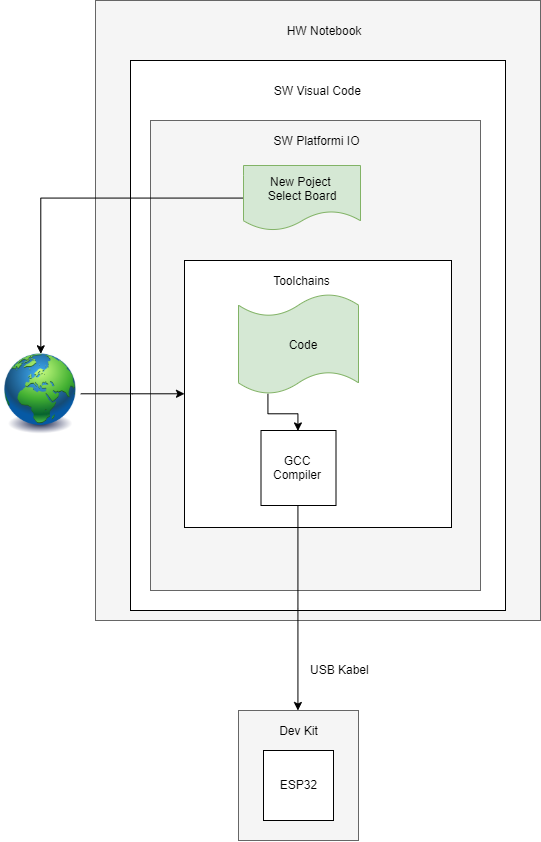
\includegraphics[width=0.8\textwidth]{graphics/DevelopDiagram.png}
	\caption{Entwicklungs Umgebung}
	\label{pic: PIO}
\end{figure} 

In diesem Projekt wurde eine Evaluation mit dem ESP-WROOM-32 Development-Board durchgeführt. Als Entwicklungsumgebung wird Visual Code von der Firma Microsoft verwendet, dies ist ein freier Quelltext-Editor, mit dem unter anderem Debugging möglich ist \cite{noauthor_visual_nodate}. In Visual Code können Extensions eingebunden werden, somit wird PlatformIO IDE \cite{platformio_platformio_nodate} kurz PIO Installiert.
PIO ist ein plattformübergreifender Code Builder und Bibliotheksmanger. Wird ein neues Projekt eröffnet, muss vom Benutzer zuerst das Entwickler Board gewählt werden, anschliessend kümmert sich PIO um die erforderlichen Toolchains, ladet diese vom Internet herunter und installiert sie. Nun kann das Developmend-Board via USB Kabel angesprochen werden. Programmcode kann kompiliert und auf den ESP32 geladen werden, sowie die Serial Port ausgaben können direkt im PIO angezeigt werden. In Abbildung \ref{pic: PIO} ist ein Blockdiagramm auf dem die Verbindungen zwischen Software und Hardware dargestellt sind.

\subsubsection{Framework Arduino}
In dem Arduino Framework erfolgt die Programmierung in C und in C++ . Das Arduino Framework steht unter der LGPL/GPL Lizenz und ist somit eine freie Software. Ein grosser Vorteil des Arduino Frameworks ist, dass zahlreiche Bibliotheken und sowie Programmcode auf  Github erhältlich sind \cite{noauthor_arduino_nodate}.

\subsubsection{Framework Zephyr}
Das Zephyr Os basiert auf einem Kernel mit geringen Platzbedarf. Da das Zephyr modular aufgebaut ist, unterstützt es mehrere Architekturen: Arm Cortex-M, Intel x86, ARC, Xtensa und noch mehr, deswegen ist es sehr universell einsetzbar. Zephyr steht unter der Apache 2.0 Lizenz \cite{noauthor_introducing_nodate}. 

\subsubsection{Framework ARM-MBED}
MBED unterstützt mit mehr als 200'000 Software Entwickler den IoT Markt. Die Grundlegende Hardware eines MBED-Geräts ist ein Arm Mikrocontroller. Ein internes Betriebssystem MBED OS bietet die Möglichkeit Hardware Komponenten anzusteuern oder mit einer Cloud zu verknüpfen. ARM-MBED steht unter der Apache 2.0 Lizenz \cite{noauthor_mbed_nodate}.

\subsubsection{Framework esp-idf}
ESP-IDF ist das offizielle Farmework für den ESP Chip. ESP-IDF steht unter der Apache Lizenz 2  \cite{noauthor_get_nodate-1} und dazugehörige Bibliotheken sind auf Github erhältlich. 

\subsubsection{Wahl Framework}
Ein geeignetes Framework für den Mikrocontroller, ist im Umfang des MCU Herstellers und mit einem Prototypen evaluiert worden. Als erste Wahl wurde das Arduino Framework genommen und ein Versuchsaufbau realisiert. Die Wahl des Arduino Framwork ist auf Grund der Programmiersprache, Verfügbarkeit und bisherigen Erfahrungen erfolgt. Ein Funktionsmuster mit Hotspot, für Grundkonfigurationen und erste MQTT-Nachrichten, konnten Erfolgreich mit dem Arduino Framework realisiert werden.

\subsubsection{Smart-Home Plattform}
\label{subsubsec: Smart-Home Plattform}
Eine Smart-Home Plattform wird benötigt, damit der Benutzer mit dem IOT-Systems interagieren kann. Doch welche Plattform ist für dieses Projekt am besten geeignet?
Angedacht ist, dass mithilfe der ausgesuchten Smart-Home-Plattform folgende Bedingungen erfüllt werden: die Plattform...\\
1. bietet Schnittstellen mit anderen Smart-Home Technologien wie KNX.\\
2. ist etabliert (grosse Community).\\
3. ist für Anfänger geeignet.\\
4. kann als Client auf vielen verschiedenen Geräten laufen.\\
5. verfügt über ein übersichtliches GUI.\\
6. hat Keine Darstellungsfehler auf verschiedenen Geräten.\\
7. Hat gewisse Vorteile gegenüber anderen Plattformen.\\
Jetzt kommt eine Analyse der Smart-Home-Plattformen. Vorgängig zu vermerken ist, dass es sich als positiv herausgestellt hat, dass alle Plattformen auf einem RasPi installiert werden können.\\
openHAB / Eclipse Smart-Home:\\
1. openHab bietet sehr viele Schnittstellen, da durch den modularen Aufbau der Architektur die flexible Anbindung neuer Technologien einfach ist. Die für dieses Projekt wichtige Bindings von Alexa und KNX sind somit vorhanden. Was ebenso interessant ist, sind konfigurierbare Features wie Dropbox Support, Google Kalender, Text to speech-Implementierung (TTS) und HABDroid. HABDroid kann wie Alexa per Sprachsteuerung Aktionen ausführen. \cite{st33zy_media_mqtt_nodate}\\
2. openHaB hat eine sehr grosse Community, wobei die ersten Smart-Home Produkte für den Massenmarkt auf Eclipse Smart-Home basierten. \cite{st33zy_media_mqtt_nodate}\\
3. Wie sich herausgestellt hat, ist die Plattform für Anfänger sehr gut zu verstehen.\\
4. openHAB kann auf jedem Endgerät installiert werden, welches Java Code ausführen kann und genügend Ressourcen hat. \cite{st33zy_media_mqtt_nodate}\\
5. Das Gui wird gestaltet durch den Anwender und so kann man sich auch ein Kachelsystem aufbauen, wenn man zu viele Kacheln hat kann es schnell Mal unübersichtlich werden.\\
6. Auf der Android App von openHab gibt unter dem Menü HABPanel Darstellungsfehler der Kacheln, so dass sie sich überlappen, was unschön ist. Jedoch müssen nicht die Kacheln im HABPanel benutzt werden, sondern es kann eine gute Menüführung mit eigens erstellten Untermenüs direkt auf dem Main Menu verwendet werden. \\
7. Die MQTT-Anbindung auf einem RasPi gestaltet sich mithilfe von openHab als besonders einfach, denn es kann nach der Installation von openHab direkt einen Broker unter openHab angelegt werden. Hierfür wird als erstes das MQTT Binding unter Add-ons installiert. Danach wird unter Inbox ein neues Gerät (MQTT Thing Binding) hinzugefügt. Das System sucht nun einen Broker, wenn er nichts gefunden hat, kann dann über manuelles Hinzufügen (add manually) einen neuen MQTT Broker hinzugefügt werden. Unter dem Konfigurationsmenü des MQTT Brokers kann unter anderem einen Namen, eine Thing ID, einen Broker Hostname, einen Username, ein Passwort sowie einen Broker Port vergeben werden. Nach der Bestätigung der Konfiguration hat man dann den Broker angelegt. In dem Menu Things kann danach ein neues Gerät hinzugefügt werden. Für das Hinzufügen kann hier MQTT Thing Binding --> manuelles hinzufügen ausgewählt werden. Nun wählt man Generic MQTT THing aus vergibt dort einen Namen und Thing ID, als Bridge wird nun der zuvor angelegte MQTT Broker ausgewählt. Nach der Bestätigung des neuen Gerätes (Thing) kann ein neuer Channel hinzugefügt werden. So kann z.B. ein Gerät welches nur ein oder aus sein muss als Channel Type On/Off Switch hinzugefügt werden. Den Channel ID und das Label können frei gewählt werden. Hier wird ebenso der MQTT state topic (für das lesen) sowie MQTT command topic (für die Befehle) eingegeben werden. Um eine Interaktion zu gewährleisten wird der Kanal mithilfe des Link Channel mit einem Item verknüpft. Unter dem Menü Control sieht man dann eine grafische Darstellung des Items hier z.B der oben genannte On/Off Switch \cite{st33zy_media_mqtt_nodate}.\\
iobroker:\\
1. Es sind Schnittstellen vorhanden jedoch weniger als bei openHAB\\
2. Ist mittlerweile ebenso etabliert, Community ist aber noch ein wenig kleiner als openHAB\\
3. iobroker bietet, wie openHAB die Möglichkeit auch ohne Programmierkentnisse bedient zu werden, jedoch kann auch Javascript angewendet werden, wodurch alle möglichen Wünsche abgedeckt werden können\cite{iobroker_einsteiger_nodate}. iobroker benötigt auf den ersten Blick sicherlich mehr Einarbeitungszeit im Gegensatz zu openHAB.\\
4. Dies ist möglich, jedoch gestaltet sich die CLient Benutzung auf dem Smartphone aufwändiger als bei openHAB\\
5. Das GUI ist sehr Individualisiert und es können mittels iobroker.vis viele eigene grafische Darstellungen erstellt werden. Jedoch sieht die Oberfläche von iobroker auf den ersten Blick "altmodisch" aus.\\
6. Es gibt soweit keine Darstellungsfehler in iobroker.\\
7. iobroker bietet mit iobroker.vis eine ein Visualisierungswerkzeug bereit, welche die Möglichkeit bietet eigene Bedienoberflächen anzulegen. Dabei können die Visualisierung alle Möglichen Komplexitätsgrade annehmen und dazu mit JavaScript verknüpft werden. Beispielsweise kann man ebenso mithilfe von JavaScript eine Schaltfläche in der Vis-Visualisierung ausführen lassen und sich eine Nachricht über Telegram verschicken \cite{korte_script_2018}.\\
Das Fazit der Analyse ist, dass openHAB einfacher zu bedienen ist und eine bessere Anbindung per Smartphone hat als iobroker. Jedoch bietet ioBroker mit iobroker.vis mächtige Werkzeuge, die Frage ist nur, ob das für dieses Projekt benötigt wird.